\chapter{Vysílání do počítačové sítě}

Pro DVBgrab potřebujeme nějaký dostatečně stabilní zdroj televizního vysílání po lokální síti. To může běžet na druhém serveru. Ale může to být i úplně nezávislé na DVBgrabu.

\vspace{10pt}
\section{DVB v České republice}

V současné době v České republice vysílají DVB signál organizace Czech Digital Group (CDG), České Radiokomunikace (CRA) a Český Telecom (CTc). Každá organizace představuje jeden multiplex, což v DVB znamená balík televizních, rozhlasových a datových kanálů, který je vysílán v rámci jedné frekvence po celém území.

Multiplex CRA je nyní zaměřen na pořady České Televize, CDG má navíc k dispozici televizi Nova, Prima, Očko, 24CZ apod., CTc mají Českou Televizi, Očko, Novu.

\section{Varianty DVB vysílání}

\begin{table}
\begin{center}
\begin{tabular}{|c|l|l|l|}
\hline
\bf{Varianta} & \bf{Použití} & \bf{Video kodek} & \bf{Modulace} \\
\hline
$DVB-T$ & pozemní & MPEG-2 & QFDM,QPSK,QAM+\\
\hline
$DVB-S$ & satelitní & MPEG-2 & QPSK+\\
\hline
$DVB-C$ & kabelové & MPEG-2 & QAM+\\
\hline
$DVB-H$ & přenosné zařízení & MPEG-4 AVC & QFDM,QPSK,QAM+\\
\hline
\end{tabular}
\end{center}
\caption{Varianty DVB vysílání}
\label{tab:tab1}
\end{table}

Variantu volíme podle dostupnosti v naší lokalitě, v Praze je nejsnazší využít variantu DVB-T.

\vspace{10pt}

Pokrytí Prahy signálem DVB-T je velmi dobré, přesto se mohou objevit problémy s použitými zesilovači, které jsou obvykle vyladěny pro zesilování frekvencí běžných pro analogové televizní vysílání a frekvence DVB-T (nad 500MHz) účinně ořezávají. Proto je v případě špatného příjmu jako první potřeba zkontrolovat použité zesilovače.

Systém, který běží na Masarykově koleji, používá signál ze 2 DVB-T karet, jedna je naladěna na multiplex CDG a druhá na CRA. 

Grabovací systém bude samozřejmě fungovat na libovolné kombinaci digitálních, ale i jinak získaných signálů, které se dají vysílat po lokální síti.

\section{Programy na vysílání}

\vspace{10pt}
Pro vysílání po síti se používají programy z projektu VideoLAN \cite{videolanURL}. Jejich použití je následující:

\vspace{10pt}

\begin{figure}[h]
\begin{center}
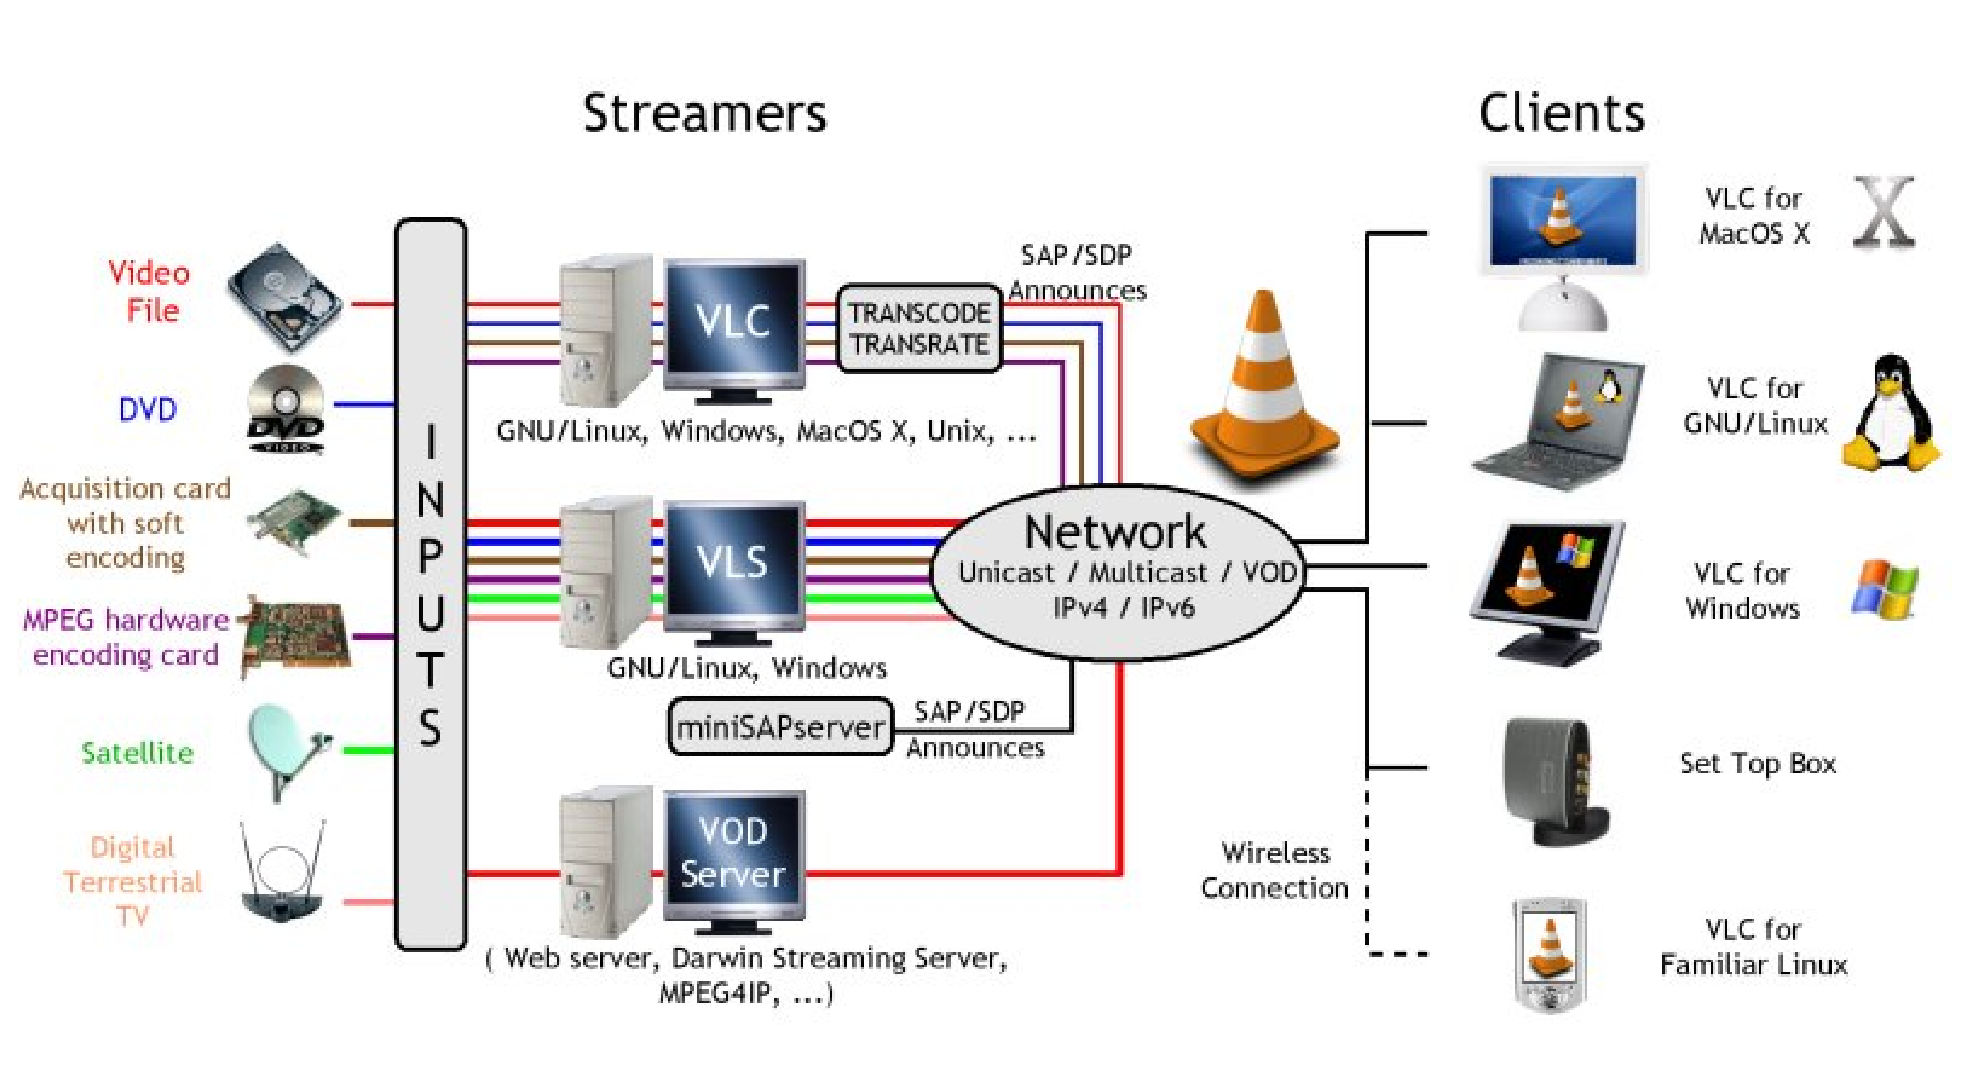
\includegraphics[width=15cm]{images/videolan.eps}
\caption{Využití programů z projektu VideoLAN}
\label{fig:videolan}
\end{center}
\end{figure}

\vspace{10pt}

\section{Potřebný hardware a ovladače}
Budeme potřebovat nějaké DVB-T karty, obvykle do slotu PCI.

Odzkoušené a ověřené jsou například karty Hauppauge WinTV-NOVA-T (Technotrend Systemtechnik GmbH Technotrend-Budget, Philips Semiconductors SAA7146 rev 01).

Pokud chceme paralelně vysílat kanály z více různých multiplexu, potřebujeme více těchto karet.

Každá DVB-T karta má potom na svém tuneru naladěnu frekvenci multiplexu a paralelně přijímá všechny kanály tohoto multiplexu.

\vspace{10pt}

Ovladače těchto karet jsou k dispozici na stránkách projektu linuxtv \cite{linuxtvURL} a také jsou součástí jádra systému řady 2.6. V novějších jádrech než je 2.6.9 se promítlo mnoho změn v ovladačích, proto je potřeba stáhnout i novější verze firmware karty, která se nahrává při načítání ovladače.

\vspace{10pt}

Pro zprovoznění vysílání je vhodné nainstalovat ještě několik uživatelských aplikací jako media-tv/linuxtv-dvb, linuxtv-dvb-apps, linuxtv-dvb-headers, libdvbpsi, dvbsnoop pro Gentoo nebo dvb-utils, dvbsnoop, dvbstream, dvbtune, libdvb-dev, libdvbpsi3, libdvbpsi3-dev pro Debian.

\section{Získání seznamu dostupných kanálů}

Získání seznamu pořadů v multiplexu popíšu již v této sekci, i když daný postup lze zjednodušit, pokud použijeme přímo VideoLanClient(VLC) místo složitější kombinace VideoLanServer(VLS)+miniSAPserver.

\vspace{10pt}

Pro zjištění dostupných kanálů lze použít například příkaz scan z balíku dvb-utils. Nejdříve je třeba připravit soubor s výchozím nastavením tuneru, aby karta věděla, ve kterém multiplexu chceme kanály vyhledávat.

\vspace{10pt}

Výchozí nastavení pro různé multiplexy lze obvykle získat z www stránek provozovatele.

\vspace{10pt}

\begin{table}
\begin{center}
\begin{tabular}{|c|l|l|l|}
\hline
\bf{Parametr} 		& \bf{Multiplex A} 	& \bf{Multiplex B} 	& \bf{Multiplex C} 	\\
			& 	\bf{CRA} 	& 	\bf{CDG} 	& 	\bf{CTC} 	\\
\hline
Typ multiplexu		&	T		&       T		&       T		\\
\hline
Frekvence v Praze	&	506 000 000	&       674 000 000	&       818 000 000	\\
\hline
Šířka pásma		&	8 MHz		&       8 MHz		&       8 MHz		\\
\hline
Vysílací mód		&	8K		&       8K		&       8K		\\
\hline
Ochranný interval 	&	1/8		&       1/16		&       1/8		\\
\hline
Kódový poměr(fec\_hi)	&	2/3		&       2/3		&       2/3		\\
\hline
Kódový poměr(fec\_lo)	&	2/3		&       1/2		&       2/3		\\
\hline
Modulace		&	64 QAM		&       64 QAM		&       64 QAM		\\
\hline
Celková bitová rychlost	&	22,12 Mbit/s	&	23,42 Mbit/s	&	22,170 Mbit/s	\\
\hline
Kódování češtiny pro EPG&	ISO 6937	&	ISO 6937	&	ISO 8859-2	\\
\hline
Hierarchický mód 	&	ne		&       ne		&       ne		\\
\hline
\end{tabular}
\end{center}
\caption{Parametry vysílání pro jednotlivé multiplexy}
\label{tab:mplexy}
\end{table}

\vspace{10pt}

Takže výchozí nastavení pak vypadá následovně (můžeme zadat všechny multiplexy najednou do jednoho souboru).

\vspace{10pt}

\begin{small}
\begin{verbatim}
# DVB-T Praha (Prague, Czech Republic)
# T freq bw fec_hi fec_lo mod transmission-mode guard-interval hierarchy
T 506000000 8MHz 2/3 2/3 QAM64 8k 1/8 NONE
T 674000000 8MHz 2/3 1/2 QAM64 8k 1/16 NONE
T 818000000 8MHz 2/3 1/2 QAM64 8k 1/8 NONE
\end{verbatim}
\end{small}

\vspace{10pt}

Výstup programu scan poté vypadá přibližně takto:
 
\vspace{10pt}

\begin{small}
\begin{verbatim}
CT1:506000000:INVERSION_AUTO:BANDWIDTH_8_MHZ:FEC_2_3:FEC_2_3:QAM_64: \
  TRANSMISSION_MODE_8K:GUARD_INTERVAL_1_8:HIERARCHY_NONE:513:641:1
CT2:506000000:INVERSION_AUTO:BANDWIDTH_8_MHZ:FEC_2_3:FEC_2_3:QAM_64: \
  TRANSMISSION_MODE_8K:GUARD_INTERVAL_1_8:HIERARCHY_NONE:514:642:2
CT24:506000000:INVERSION_AUTO:BANDWIDTH_8_MHZ:FEC_2_3:FEC_2_3:QAM_64: \
  TRANSMISSION_MODE_8K:GUARD_INTERVAL_1_8:HIERARCHY_NONE:515:643:3
Nova:506000000:INVERSION_AUTO:BANDWIDTH_8_MHZ:FEC_2_3:FEC_2_3:QAM_64: \
  TRANSMISSION_MODE_8K:GUARD_INTERVAL_1_8:HIERARCHY_NONE:516:644:4
Praha:506000000:INVERSION_AUTO:BANDWIDTH_8_MHZ:FEC_2_3:FEC_2_3:QAM_64: \
  TRANSMISSION_MODE_8K:GUARD_INTERVAL_1_8:HIERARCHY_NONE:0:658:18
Vltava:506000000:INVERSION_AUTO:BANDWIDTH_8_MHZ:FEC_2_3:FEC_2_3:QAM_64: \
  TRANSMISSION_MODE_8K:GUARD_INTERVAL_1_8:HIERARCHY_NONE:0:659:19
D-dur:506000000:INVERSION_AUTO:BANDWIDTH_8_MHZ:FEC_2_3:FEC_2_3:QAM_64: \
  TRANSMISSION_MODE_8K:GUARD_INTERVAL_1_8:HIERARCHY_NONE:0:661:21
Leonardo:506000000:INVERSION_AUTO:BANDWIDTH_8_MHZ:FEC_2_3:FEC_2_3:QAM_64: \
  TRANSMISSION_MODE_8K:GUARD_INTERVAL_1_8:HIERARCHY_NONE:0:662:22
Radio Cesko:506000000:INVERSION_AUTO:BANDWIDTH_8_MHZ:FEC_2_3:FEC_2_3:QAM_64: \
  TRANSMISSION_MODE_8K:GUARD_INTERVAL_1_8:HIERARCHY_NONE:0:663:23
\end{verbatim}
\end{small}

\vspace{10pt}

pro České Radiokomunikace

\vspace{10pt}

a

\vspace{10pt}

\begin{small}
\begin{verbatim}
CT 1:674000000:INVERSION_AUTO:BANDWIDTH_8_MHZ:FEC_2_3:FEC_1_2:QAM_64: \
  TRANSMISSION_MODE_8K:GUARD_INTERVAL_1_16:HIERARCHY_NONE:2501:2502:5
CT 2:674000000:INVERSION_AUTO:BANDWIDTH_8_MHZ:FEC_2_3:FEC_1_2:QAM_64: \
  TRANSMISSION_MODE_8K:GUARD_INTERVAL_1_16:HIERARCHY_NONE:164:96:4
NOVA:674000000:INVERSION_AUTO:BANDWIDTH_8_MHZ:FEC_2_3:FEC_1_2:QAM_64: \
  TRANSMISSION_MODE_8K:GUARD_INTERVAL_1_16:HIERARCHY_NONE:205:206:3
TOP TV:674000000:INVERSION_AUTO:BANDWIDTH_8_MHZ:FEC_2_3:FEC_1_2:QAM_64: \
  TRANSMISSION_MODE_8K:GUARD_INTERVAL_1_16:HIERARCHY_NONE:2601:2602:2
CT24:674000000:INVERSION_AUTO:BANDWIDTH_8_MHZ:FEC_2_3:FEC_1_2:QAM_64: \
  TRANSMISSION_MODE_8K:GUARD_INTERVAL_1_16:HIERARCHY_NONE:1026:1027:7
CRo 2:674000000:INVERSION_AUTO:BANDWIDTH_8_MHZ:FEC_2_3:FEC_1_2:QAM_64: \
  TRANSMISSION_MODE_8K:GUARD_INTERVAL_1_16:HIERARCHY_NONE:0:2832:6
CRo 1:674000000:INVERSION_AUTO:BANDWIDTH_8_MHZ:FEC_2_3:FEC_1_2:QAM_64: \
  TRANSMISSION_MODE_8K:GUARD_INTERVAL_1_16:HIERARCHY_NONE:0:2831:9
Proglas:674000000:INVERSION_AUTO:BANDWIDTH_8_MHZ:FEC_2_3:FEC_1_2:QAM_64: \
  TRANSMISSION_MODE_8K:GUARD_INTERVAL_1_16:HIERARCHY_NONE:0:180:11
Evropa 2:674000000:INVERSION_AUTO:BANDWIDTH_8_MHZ:FEC_2_3:FEC_1_2:QAM_64: \
  TRANSMISSION_MODE_8K:GUARD_INTERVAL_1_16:HIERARCHY_NONE:0:110:19
EXPRESRADIO:674000000:INVERSION_AUTO:BANDWIDTH_8_MHZ:FEC_2_3:FEC_1_2:QAM_64: \
  TRANSMISSION_MODE_8K:GUARD_INTERVAL_1_16:HIERARCHY_NONE:0:120:22
CLASSIC FM:674000000:INVERSION_AUTO:BANDWIDTH_8_MHZ:FEC_2_3:FEC_1_2:QAM_64: \
  TRANSMISSION_MODE_8K:GUARD_INTERVAL_1_16:HIERARCHY_NONE:0:130:23
Prima:674000000:INVERSION_AUTO:BANDWIDTH_8_MHZ:FEC_2_3:FEC_1_2:QAM_64: \
  TRANSMISSION_MODE_8K:GUARD_INTERVAL_1_16:HIERARCHY_NONE:161:84:1
\end{verbatim}
\end{small}

\vspace{10pt}

pro Czech Digital Group 

\vspace{10pt}

MPEG-2 transport stream je balíkem elementárních kanálů (MPEG-2 ES - Elementary stream) a informačních tabulek.

Každá složka je jednoznačně určena identifikačním číslem PID (13 bitové identifikační číslo složky, unikátní v rámci multiplexu). Podle PID se určuje, které pakety patří k sobě.

\vspace{10pt}

\textbf{PAT - Program Association Table} je první informační tabulkou, která je vždy vysílána s PID 0x0. Obsahuje pro každý kanál v multiplexu PID, kde je vysílána jeho PMT tabulka.

\textbf{PMT - Program Map Table} je potom seznam PID jednotlivých složek, každý kanál má vysílánu vlastní PMT tabulku na vlastním PID.

\textbf{PCR - Program Clock Reference} zdroj časového signálu pro dekodér.

Na vyhrazeném \textbf{PIDu 0x1FFF} mohou být ještě vysílány prázdné pakety, které slouží jenom na doplnění vysílání do určité velikosti, aby byla dodržena konstantní velikost (constant bitrate).

\vspace{10pt}

Příkaz scan nám tedy vypsal informační tabulky PAT a PMT. Každý řádek je tedy jednou tabulkou PMT. V prvním sloupci je název kanálu, poté jsou parametry společné pro celý multiplex a zajímavé jsou pak poslední číselné sloupce oddělené dvojtečkou.

\vspace{10pt}

Úplně poslední určuje PID této PMT tabulky = identifikátor kanálu.
Předcházející čísla jsou PID jednotlivých složek programu a to v pořadí video, audio.

\vspace{10pt}

Přehledně je to zobrazeno na následujícím obrázku \ref{fig:PATaPMT}, převzatém z \cite{digitvURL}.

\vspace{10pt}

\begin{figure}[ht]
\begin{center}
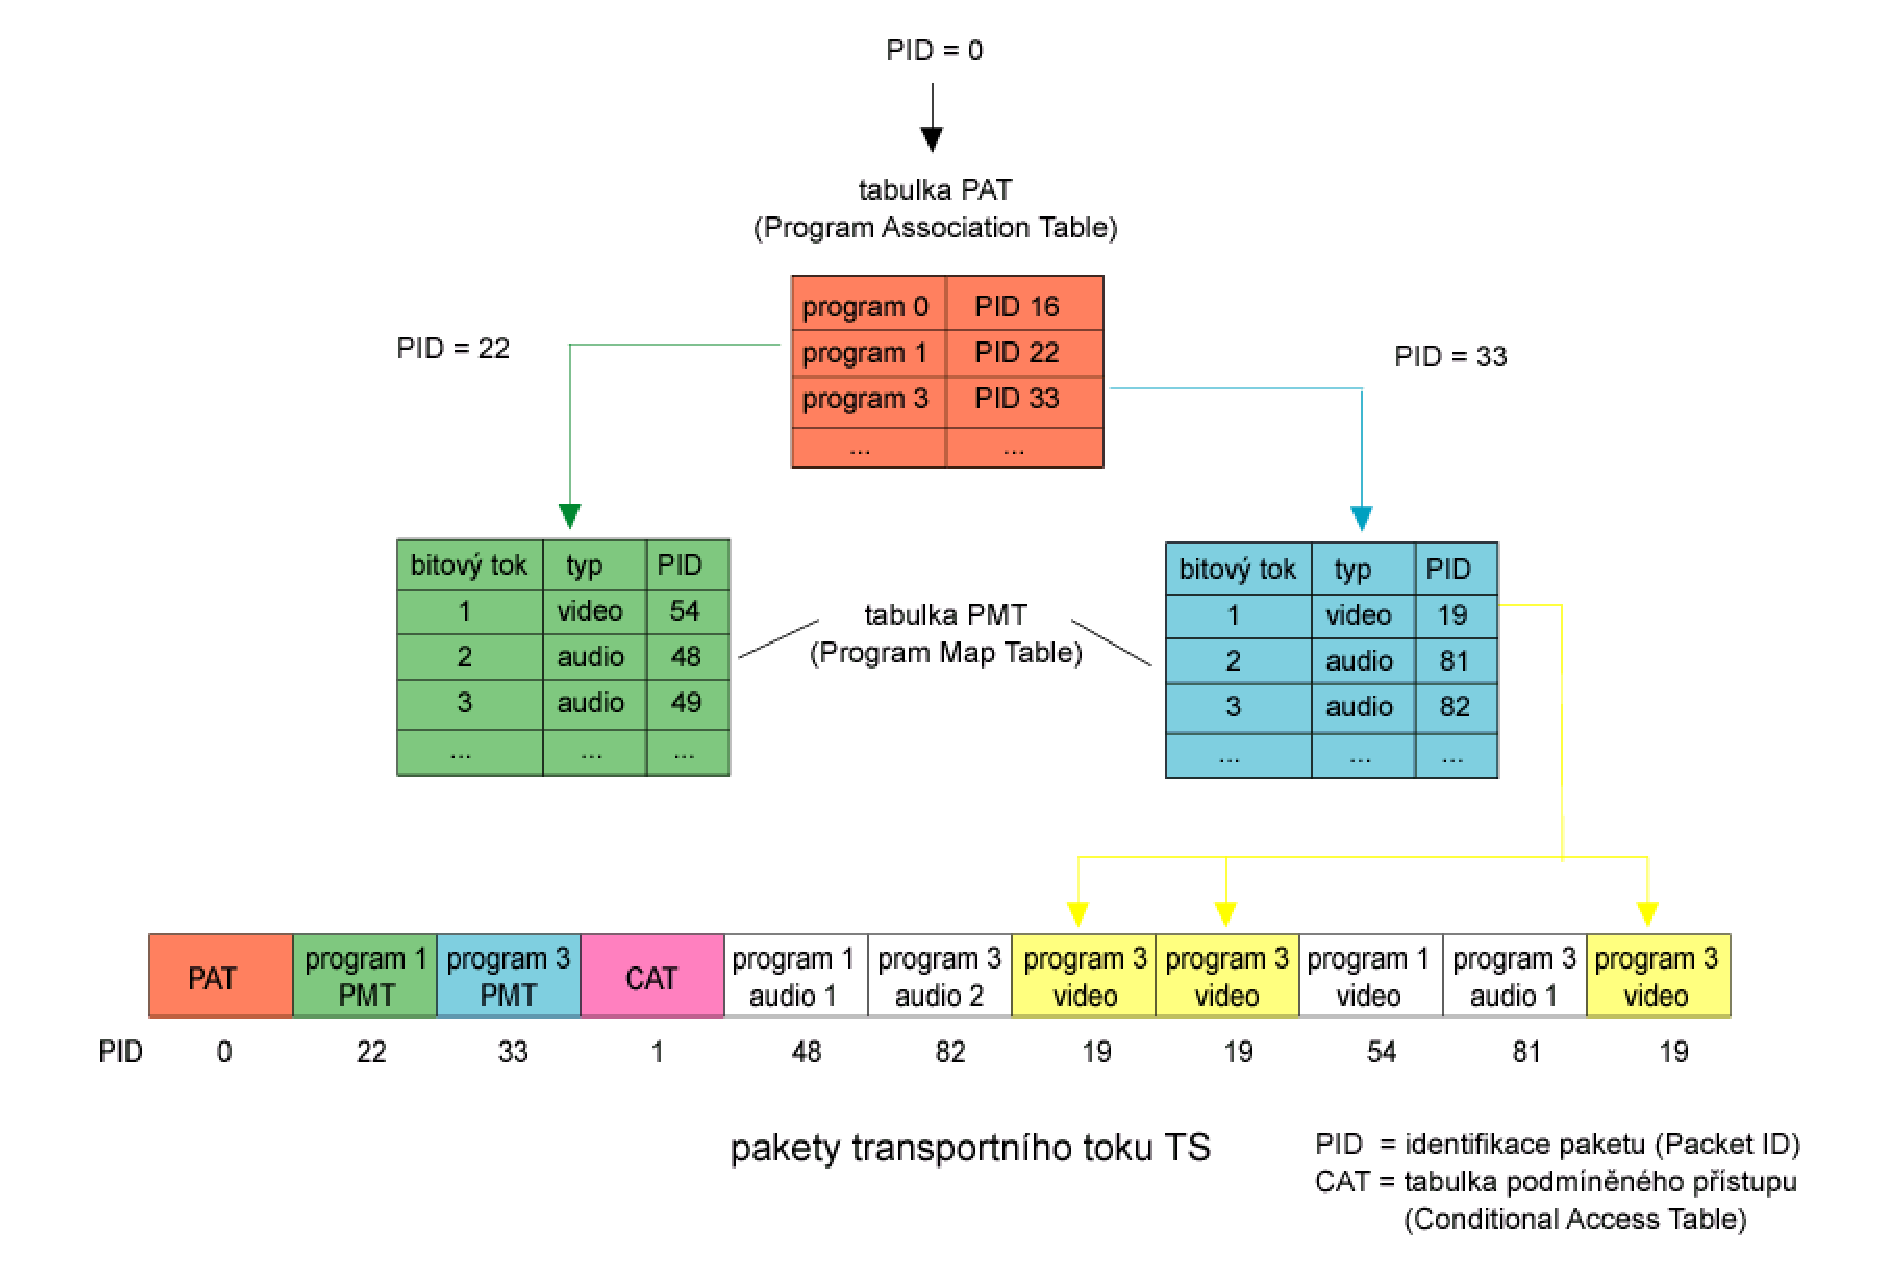
\includegraphics[width=15cm]{images/PATaPMT.eps}
\caption{Tabulky toků v MPEG-2}
\label{fig:PATaPMT}
\end{center}
\end{figure}

\section{Metody vysílání}

\vspace{10pt}

Nyní tedy umíme zjistit dostupné kanály a jejich konfiguraci. Před volbou vysílacího serveru se ještě musíme rozhodnout pro metodu vysílání.
Pro provozování DVBgrabu je nejdůležitější vysílání pomocí multicastu. Multicast je totiž nejefektivnější a díky tomu vlastně jediný použitelný pro větší lokální sítě. 

\vspace{10pt}

\begin{bf}$Unicast$\end{bf}


\begin{bf}Popis:\end{bf} vysílání pro konkrétní IP adresu


\begin{bf}Výhody:\end{bf} snadná konfigurace pro málo uživatelů, možnost definovat povolené adresy


\begin{bf}Nevýhody:\end{bf} data se posílají tolikrát, kolik je uživatelů, značně zatěžuje síť

\vspace{10pt}

\begin{bf}$Multicast$\end{bf}


\begin{bf}Popis:\end{bf} vysílání pro skupinu IP adres


\begin{bf}Výhody:\end{bf} do skupiny se klient může přihlašovat a odhlašovat pomocí IGMP paketů, takže dostává data jen z těch stanic, které sleduje


\begin{bf}Nevýhody:\end{bf} pro funkční a efektivní multicast vysílání je potřeba, aby switche podporovali IGMP snooping, což je mechanismus přeposílání packetů pouze na ty porty, ze kterých přišel přihlašovací paket do dané skupiny, jinak se to šíří v rámci switche jako broadcast

\vspace{10pt}

\begin{bf}$Broadcast$\end{bf}
   

\begin{bf}Popis:\end{bf} vysílání na úplně všechny IP v síti
 

\begin{bf}Výhody:\end{bf} snadné


\begin{bf}Nevýhody:\end{bf} značné zatížení sítě, data dostávají všichni a ze všech stanic

\vspace{10pt}

\section{Seznam kanálů pro uživatele}

Když máme seznam pořadů a přidělíme jim adresy, na kterých je budeme vysílat, je vhodné vytvořit také statický playlist. Ten se bude hodit uživatelům, kteří nebudou používat přehrávač s podporou SAP playlistu. Playlist M3U je obyčejný textový soubor obvykle s příponou .m3u obsahující pro každý pořad jeho název (za EXTINF) a adresu (následující řádek), viz ukázka:

\vspace{10pt}

\begin{small}
\begin{verbatim}
#EXTM3U
#EXTINF:0,CRA_CT1
rtp://@239.194.12.1
...
#EXTINF:0,CRA6_CT1
rtp://@[ff08::701]
...
\end{verbatim}
\end{small}

\vspace{10pt}

\section{VideoLAN Server nebo VideoLAN Client?}

Pro vysílání můžeme použít buď VLS (VideoLan Server) nebo VLC (VideoLan Client). Zásadní rozdíl je ve složitosti konfigurace a udržovanosti projektu. VLS není již několik let aktivně vyvíjen, VLC už podporuje všechny jeho funkce a nyní i mnohem více.

\vspace{10pt}

VLS má složitějsí konfiguraci, kde je potřeba definovat správně seznam kanálů pro jednotlivé karty v souborech .dvbrc.N. Také neobsahuje integrovaný SAP server jako VLC. To pro nás znamená další práci s konfigurací SAP serveru. Vlastní konfigurace v souboru vls.cfg je sice přehledná, ale přesto dost náchylná k chybám při úpravách. Velkou výhodou VLS je při použití na serverech bez grafického prostředí, protože ani jeho binární balíčky nezávisejí na žádných grafických knihovnách.

\vspace{10pt}

VLC má mnohem snažší konfiguraci, nepodporuje .dvbrc.N soubory (což sice znamená, že nemůžeme definovat pro programy symbolické názvy, ale taky to ušetří práci s vytvářením těchto souborů, pokud se skladba programů v multiplexu častěji mění). Má integrovaný SAP server, takže je vše schováno přehledně v jednom souboru. Nevýhoda u binárních instalačních balíčků se dá obejít buď překompilováním VLC do balíčku bez podpory X serveru nebo například u distribuce Gentoo je to jen o správné volbě USE flagů při instalaci.

\section{Popis VideoLAN Serveru}

Open source projekt, který umí vysílat do sítě mnoha různými způsoby a z mnoha různých zdrojů.

\vspace{10pt}

\textbf{Zdroje}

\vspace{10pt}

statické soubory na disku nebo nějakém médiu (ve formátu MPEG-1, MPEG-2, MPEG-4),

disky DVD v DVD mechanikách,

digitální satelitní vysílání z DVB-S karet,

digitální pozemní vysílání z DVB-T karet,

přímé přenosy z kamery nebo komprimační karty

\vspace{10pt}

\textbf{Výstupy}

\vspace{10pt}

na konkrétní IP adresu - unicast

na všechny adresy v určité síti - broadcast

na všechny počítače, které se přihlásí k odběru dané skupiny - multicast

a to vše jak ve variantě IPv4, tak v modernější IPv6

\vspace{10pt}

Hardwarové nároky jsou přibližně Pentium 100 MHz a 32MB RAM pro vysílání jednoho televizního kanálu. Pokud jsou vysílány data ze souborů na lokálním disku, tak je větším omezením čtecí rychlost disku a síťové připojení.

\vspace{10pt}

VLS lze používat jak ve verzi pro MS Windows, tak pro Linux. K dispozici jsou samozřejmě i zdrojové kódy.

\vspace{10pt}

Instalační binární i zdrojové balíčky jsou ke stažení na adrese \cite{videolanURL}.
Linuxové distribuce obvykle obsahují předpřipravené instalační balíčky (například Gentoo a Debian mají). 

\vspace{10pt}

\section{Konfigurace VideoLAN Serveru}
\vspace{10pt}

Tady budeme potřebovat znát PID tabulek PMT pro všechny programy, to bylo popsáno ve zvláštní sekci.

Tyto údaje potřebujeme zkonvertovat do formátu konfiguračního souboru kanálů pro VLS (.dvbrc). Tyto soubory obsahují na prvních řádcích definici multiplexu a jeho parametrů viz. tabulka \ref{tab:mplexy}. Pak každý kanál má nastaveno jméno v parametru NAME a poté v SID je identifikační číslo toku s odpovídající tabulkou PMT.

Takže výsledek vypadá asi takto:

\vspace{10pt}

\begin{small}
\begin{verbatim}
LNB ID 1 TYPE 2
  SAT ID 1 NAME "DVBT-Cra" LNBID 1 FMIN 150000000 FMAX 778000000
    TRANSPONDER ID 1 SATID 1 TYPE 2 FREQ 506000000 BANDWIDTH 0 HP_RATE 2 \
     LP_RATE 6 MODULATION 1 TRANSMISSION_MODE 1 GUARD_INTERVAL 2 HIERARCHY 0
      CHANNEL ID 1 NAME "cra_ct1" SATID 1 TPID 1 SID 1 TYPE 0
      CHANNEL ID 2 NAME "cra_ct2" SATID 1 TPID 1 SID 2 TYPE 0
      CHANNEL ID 3 NAME "cra_ct24" SATID 1 TPID 1 SID 3 TYPE 0
      CHANNEL ID 4 NAME "cra_nova" SATID 1 TPID 1 SID 4 TYPE 0
      CHANNEL ID 5 NAME "cra_praha" SATID 1 TPID 1 SID 18 TYPE 0
      CHANNEL ID 6 NAME "cra_vltava" SATID 1 TPID 1 SID 19 TYPE 0
      CHANNEL ID 7 NAME "cra_ddur" SATID 1 TPID 1 SID 21 TYPE 0
      CHANNEL ID 8 NAME "cra_leonardo" SATID 1 TPID 1 SID 22 TYPE 0
      CHANNEL ID 9 NAME "cra_cesko" SATID 1 TPID 1 SID 23 TYPE 0
\end{verbatim}
\end{small}

\vspace{10pt}

pro České Radiokomunikace 

\vspace{10pt}

a

\vspace{10pt}

\begin{small}
\begin{verbatim}
LNB ID 1 TYPE 2
  SAT ID 1 NAME "DVBT-Cdg" LNBID 1 FMIN 150000000 FMAX 778000000
    TRANSPONDER ID 0001 SATID 0001 TYPE 2 FREQ 674000000 BANDWIDTH 0 HP_RATE 2 \
     LP_RATE 6 MODULATION 1 TRANSMISSION_MODE 1 GUARD_INTERVAL 2 HIERARCHY 0
      CHANNEL ID 1 NAME "cdg_prima" SATID 1 TPID 1 SID 1 TYPE 0
      CHANNEL ID 2 NAME "cdg_top" SATID 1 TPID 1 SID 2 TYPE 0
      CHANNEL ID 3 NAME "cdg_nova" SATID 1 TPID 1 SID 3 TYPE 0
      CHANNEL ID 4 NAME "cdg_ct2" SATID 1 TPID 1 SID 4 TYPE 0
      CHANNEL ID 5 NAME "cdg_ct1" SATID 1 TPID 1 SID 5 TYPE 0
      CHANNEL ID 6 NAME "cdg_cro2" SATID 1 TPID 1 SID 6 TYPE 0
      CHANNEL ID 7 NAME "cdg_ct24" SATID 1 TPID 1 SID 7 TYPE 0
      CHANNEL ID 8 NAME "cdg_cro1" SATID 1 TPID 1 SID 9 TYPE 0
      CHANNEL ID 9 NAME "cdg_proglas" SATID 1 TPID 1 SID 11 TYPE 0
      CHANNEL ID 10 NAME "cdg_e2" SATID 1 TPID 1 SID 19 TYPE 0
      CHANNEL ID 11 NAME "cdg_expres" SATID 1 TPID 1 SID 22 TYPE 0
      CHANNEL ID 12 NAME "cdg_classic" SATID 1 TPID 1 SID 23 TYPE 0
\end{verbatim}
\end{small}

\vspace{10pt}

pro Czech Digital Group.

\vspace{10pt}

Tyto dva soubory pojmenujeme .dvbrc pro první DVB kartu a .dvbrc.1 pro druhou. Soubory uložíme do domovského adresáře uživatele, pod kterým budeme chtít VLS spouštět. Pravděpodobně vytvoříme speciálního neprivilegovaného uživatele, např. vls s domovským adresářem /var/lib/vls.

\vspace{10pt}

Vlastní konfigurační soubor VLS je obvykle /etc/videolan/vls.conf. 

\vspace{10pt}

Na začátku obsahuje společné nastavení jako telnet rozhraní pro správu vls po spuštění. Tato část myslím nepotřebuje dodatečný komentář.

\vspace{10pt}

\begin{small}
\begin{verbatim}
#
# Nastavení aplikace
#
BEGIN "Vls"
  LogFile       = "/var/log/vls"        # log soubor
  ScreenLog     = "disable"             # logovat na obrazovku
  SystemLog     = "enable"              # logovat do systémového logu
END

#
# Povolené příkazy pro telnetové uživatele
#
BEGIN "Groups"
  monitor       = "help|browse|logout"
  master        = "help|browse|start|resume|suspend|stop \
                   |shutdown|logout|config|program|input|channel|show"
END

#
# Uživatelé pro telnet
#
BEGIN "Users"
  monitor       = "3BcKWoiQn0vi6:monitor"       # heslo nastaveno na 'monitor'
  master        = "JKg2TpPerilnw:master"        # heslo nastaveno na 'bozo'
END

#
# Nastavení telnet rozhraní
#
BEGIN "Telnet"
  Domain        = "Inet4"              # Inet4 nebo Inet6
  LocalAddress  = "127.0.0.1"          # Adresa lokálního rozhraní
  LocalPort     = "9999"               # Použitý port
  Use           = "true"               # Povolit telnet
END
\end{verbatim}
\end{small}

\vspace{10pt}

Dále je obsažena definice zdrojů dat a jejich konfigurace.

\vspace{10pt}

\begin{small}
\begin{verbatim}
#
# Zdroje toků dat
#
BEGIN "Inputs"
  dvb0          = "dvb"                 # Video výstup z první DVB karty, 
                                        # odpovídá .dvbrc souboru
  dvb1          = "dvb"                 # Video výstup z druhé DVB karty, 
                                        # odpovídá .dvbrc.1 souboru
END

#
# Konfigurace video vstupů
#
BEGIN "dvb0"                           # Multiplex A CRA
  Frequency = "506000000"              # Frekvence
  DeviceNumber = "0"                   # Zařízení /dev/dvb/adapter<i>
  SendMethod   = "0"                   # 0 - Posílat všechny toky k danému programu, 
                                       # 1 - posílat jen MPEG2 data
  IgnoreTimeout = "1"                  # Ignorovat timeout
  TrickPlay = "normal"                 
END
BEGIN "dvb1"                           # Multiplex B CDG
  Frequency = "674000000"              # Frekvence
  DeviceNumber = "1"                   # Zařízení /dev/dvb/adapter<i>
  SendMethod   = "0"                   # 0 - Posílat všechny toky k danému programu, 
                                       # 1 - posílat jen MPEG2 data
  IgnoreTimeout = "1"                  # Ignorovat timeout
  TrickPlay = "normal"
END
\end{verbatim}
\end{small}

\vspace{10pt}

Definice distribučních kanálů - nejdříve je v sekci Channels seznam distribučních kanálů a pak má každý svou sekci s konfigurací. Na ukázku jsou zobrazeny varianty jak pro použití IPv4, tak IPv6.

\vspace{10pt}

\begin{small}
\begin{verbatim}
#
# Seznam distribučních kanálů
#
BEGIN "Channels"
  mcra_ct1        = "network"
  mcra6_ct1       = "network"
...
END
#
# Konfigurace distribučních kanálů
#
BEGIN "mcra_ct1"               # Program CT1 z multiplexu CRA přes IPv4
  Type      = "multicast"      # Medota vysílání je multicast
  TTL       = "1"              # Dosah vysílání je pouze po nejbližší 
                               # router (pouze vnitřní síť)
  DstHost   = "239.194.12.1"   # Multicastova IP adresa, 
                               # identifikátor multicast skupiny
  DstPort   = "1234"           # Port
  Interface = "eth0"           # Přes které síťové rozhraní chceme posílat data
END
BEGIN "mcra6_ct1"              # Program CT1 z multiplexu CRA přes IPv6
  Domain    = "inet6"          # Typ IPv6
  Type      = "multicast"      # Medota vysílání je multicast
  TTL       = "1"              # Dosah vysílání je pouze po nejbližší 
                               # router (pouze vnitřní síť)
  DstHost   = "ff08::701"      # Multicastova IP adresa, 
                               # identifikátor multicast skupiny
                               # ff08 značí lokální multicast v ramci místní sítě a 
                               # 701 je identifikátor skupiny
  DstPort   = "1234"           # Port
  Interface = "eth0"           # Přes které síťové rozhraní chceme posílat data
END
...

\end{verbatim}
\end{small}

\vspace{10pt}

A nakonec ještě seznam příkazů pro spouštění vysílání při startu VLS. Parametr --rtp zajišťuje vysílání pomocí protokolu rtp, který obsahuje proti UDP navíc synchronizační údaje a díky tomu pak vysílání jde přehrávat i MPlayerem.

\vspace{10pt}

\begin{small}
\begin{verbatim}
#
# Příkazy po spuštění
#
BEGIN "LaunchOnStartUp"
  command0  = "start cra_ct1 mcra_ct1 dvb0 --rtp"
   # Spuštění programu ČT1 (v .dvbrc musí být přesně cra_ct1) ze zdroje dvb0 
   # přes distribuční kanál mcra_ct1
  command1  = "start cra_ct1 mcra6_ct1 dvb0 --rtp"   
   # Spuštění programu ČT1 (v .dvbrc musí být přesně cra_ct1) ze zdroje dvb0 
   # přes distribuční kanál mcra6_ct1
...
END

\end{verbatim}
\end{small}

\vspace{10pt}

VLS je skvělý program pro serverové použití, nepotřebuje grafické knihovny, jeho konfigurace je přehledná. Vývoj jde ale rychleji kupředu v podobném projektu ze stejné dílny, který je zároveň jak klientským prohlížečem, tak streamovacím serverem. Tento produkt se jmenuje VideoLAN Client.

\vspace{10pt}

\section{Mini SAP server}

Opět open source projekt, SAP (Session Announcement Protocol) je protokol pro oznamování změn ve skladbě vysílání. 

\vspace{10pt}

Uživatelé mohou zvolit 2 přístupy. Buď použijí staticky vygenerovaný soubor .m3u, který obsahuje seznam kanálů, které v síti vysíláme, ale při každé změně musíme aktualizovat .m3u soubor a uživatelé si musí stáhnout někde aktuální verzi.

\vspace{10pt}

Druhá možnost je použít tento protokol (jak na straně serveru tak klienta). V konfiguraci serveru pro tento protokol je opět seznam kanálů, které vysíláme, ale pokaždé, když provedeme změnu, tak se tato změna projeví ihned i všem uživatelům, kteří mají nastaveno používání playlistu získaného ze SAP protokolu.

\vspace{10pt}

SAP server periodicky vysílá aktuální playlist také pomocí multicast vysílání, podporuje jak IPv4, tak IPv6 variantu.

\vspace{10pt}

Mini-SAP-server lze provozovat pod operačním systémem Linux a Mac OS X. 

\vspace{10pt}

Instalace je snadná, po stažení zdrojových kódů by měla stačit obvyklá sekvence ./configure \&\& make \&\& make install. A možná bude k dispozici i instalační balík přímo z distribuce.

\vspace{10pt}

Konfigurace je celkem přímočará, v souboru /etc/sap.cfg má každý kanál svou sekci viz. ukázka: 

\vspace{10pt}

\begin{small}
\begin{verbatim}
[program]                               # začátek sekce
type=rtp                                # protokol vysílání RTP
name=CRA CT1                            # název kanálu zobrazovaný uživateli
user=Masarka                            # jméno subjektu, který kanál vysílá
machine=zeus.mk.cvut.cz                 # jméno serveru, ze kterého je kanál vysílán
playlist_group=Masarka                  # složka, do které se daný kanál zařadí
site=http://dvbgrab.mk.cvut.cz/stream   # stránky s informacemi o vysílání
address=239.194.12.1                    # IP adresa pro přihlášení kanálu
port=1234                               # port, na který jsou posílána data
program_ttl=32                          # TimeToLive multicast paketů
program_ipversion=4                     # použitá verze IP protokolu
\end{verbatim}
\end{small}

\vspace{10pt}

Mini SAP Server je velmi snadno použitelný a pro uživatele velmi pohodlný doplněk vysílání. VLC má vysílání SAP informací dokonce zabudováno.

\vspace{10pt}

\section{Popis VideoLAN Client}

Další projekt s otevřeným kódem, který podporuje mnoho platforem: Linux, Windows, Mac OS X, BeOS, *BSD, Solaris, Familiar Linux, Yopy/Linupy and QNX. VLC nepracuje na Mac OS\ 9 a pravděpodobně ani nikdy nebude.

\vspace{10pt}

\textbf{Umí přehrávat}

soubory z disků a mechanik (formáty MPEG-1, MPEG-2, MPEG-4/DivX apod.)

DVD disky, VCD soubory

ze satelitních/pozemních karet digitálního vysílání DVB-S/DVB-T

z analogových karet přes rozhraní v4l(video for linux)

\vspace{10pt}

\textbf{Umí také vysílat stejně jako VLS.}

\vspace{10pt}

Instalace je velmi snadná. K dispozici jsou instalační balíky pro mnoho operačních systémů.

\vspace{10pt}

Konfigurace klienta obecně není potřeba. 

\vspace{10pt}

VLC je nejspolehlivějším přehrávačem pro přehrávání záznamů z DVBgrabu v prostředí Microsoft Windows, protože je založen na stejné implementaci kodeků FFmeg/libavcodec jako komprimační nástroj mencoder.

Trošku pohodlí může přidat vytvoření zástupce/skriptu, který při spuštění načte námi používaný statický playlist z .m3u souboru a zapne podporu získávání playlistu ze SAP událostí. Klienti si uloží staticky playlist do svého domovského adresáře jako .vlc.m3u a pak do definice Cíl v zástupci ve windows resp. do nějakého startovacího skriptu v linuxu přidají parametr -S sap pro podporu SAP playlistu a nakonec přidají cestu k uloženému souboru .m3u. VLC pak po startu hned obsahuje použitelný playlist ze souboru a po nějaké prodlevě se doplní ještě SAP playlist.

\vspace{10pt}

\begin{small}
\begin{verbatim}
C:\Program Files\VideoLAN\vlc.exe -S sap %%HOMEPATH%%/.vlc.m3u
resp.
/usr/bin/vlc -S sap ~/.vlc.m3u
\end{verbatim}
\end{small}

\vspace{10pt}

\section{Konfigurace VideoLAN Client pro použití na vysílání do sítě}

\vspace{10pt}

Aby nám na serveru, který nemusí obsahovat vůbec grafické prostředí, nechtěl VLC vytvářet grafické okno aplikace, tak používáme režim provozu VideoLAN Manager (VLM). Veškerá konfigurace je v jednom souboru, který uložíme například do /etc/videolan/vlm/vlm.cfg.

\vspace{10pt}

\begin{small}
\begin{verbatim}
# Vytvoření nového zdroje dat
new CRA broadcast enabled

# Nastavíme typ zdroje na DVB
setup CRA input dvb:

# Nastavení DVB parametrů viz. tabulka.
setup CRA option dvb-adapter=0
setup CRA option dvb-frequency=506000000
setup CRA option dvb-bandwidth=8
setup CRA option dvb-transmission=8
setup CRA option dvb-guard=8
setup CRA option dvb-hierarchy=-1
setup CRA option dvb-modulation=64

# Chceme data nechávat v transport streamu a 
# posílat je po jednotlivých programech
setup CRA option ts-es-id-pid

# Seznam identifikačních čísel programů, které nás zajímají
setup CRA option programs=1,2,3,4,5,10,11,12,13,14,15,16,1000

# Nastavení výstupů

# Použijeme modul duplicate, který z multiplexu vybere toky
# odpovídající programu podle klauzule select a ty pošle i
# do modulu std, který je definován v klauzuli dst

# std modul nastavíme pro typ vysílání rtp, mux=ts znamená
# nekonvertovat, v url je multicastová IP a port

# sap zajistí vysílání SAP událostí pro daný program,
# group a name pak udávají, jak se bude program
# zobrazovat v klientu po povolení SAP playlistu

setup CRA output #duplicate
{
dst=std{access=rtp,mux=ts,url=239.194.12.1:1234, \
  sap,group="Masarka-CRA",name="CT1"},select="program=1"
,dst=std{access=rtp,mux=ts,url=239.194.12.2:1234, \
  sap,group="Masarka-CRA",name="CT2"},select="program=2"
,dst=std{access=rtp,mux=ts,url=239.194.12.3:1234, \ 
  sap,group="Masarka-CRA",name="CT24"},select="program=3"
,dst=std{access=rtp,mux=ts,url=239.194.12.4:1234, \
  sap,group="Masarka-CRA",name="CT4"},select="program=4"
,dst=std{access=rtp,mux=ts,url=239.194.12.5:1234, \
  sap,group="Masarka-CRA",name="Nova"},select="program=5"
,dst=std{access=rtp,mux=ts,url=239.194.12.6:1234, \
  sap,group="Masarka-CRA",name="CRO1"},select="program=10"
,dst=std{access=rtp,mux=ts,url=239.194.12.7:1234, \
  sap,group="Masarka-CRA",name="CRO2"},select="program=11"
,dst=std{access=rtp,mux=ts,url=239.194.12.8:1234, \
  sap,group="Masarka-CRA",name="CRO3"},select="program=12"
,dst=std{access=rtp,mux=ts,url=239.194.12.9:1234, \
  sap,group="Masarka-CRA",name="CRO4"},select="program=13"
,dst=std{access=rtp,mux=ts,url=239.194.12.10:1234, \
  sap,group="Masarka-CRA",name="Ddur"},select="program=14"
,dst=std{access=rtp,mux=ts,url=239.194.12.11:1234, \
  sap,group="Masarka-CRA",name="Leonardo"},select="program=15"
,dst=std{access=rtp,mux=ts,url=239.194.12.12:1234, \
  sap,group="Masarka-CRA",name="Cesko"},select="program=16"
,dst=std{access=rtp,mux=ts,url=239.194.12.13:1234, \
  sap,group="Masarka-CRA",name="MHP"},select="program=1000"
}
\end{verbatim}
\end{small}

\vspace{10pt}

Spouštění po startu zajistíme například přidáním spouštěcího skriptu do /etc/init.d/vlm, který pouze načte konfiguraci např. z /etc/sysconfig/dvb.

\vspace{10pt}

\begin{small}
\begin{verbatim}
VLM_CONFIG_FILE=/etc/videolan/vlm/vlm.cfg
VLM_LOG_FILE=/var/log/vlm.log
VLM_TELNET_PORT=7777
VLM_TELNET_PASSWORD=password
\end{verbatim}
\end{small}

\vspace{10pt}

a pak spustí VLC v režimu VLM (VideoLAN Manager) pouze s telnetovým rozhraním.

\vspace{10pt}

\begin{small}
\begin{verbatim}
VLCSERVER=/usr/bin/vlc
daemon --user vlc "$VLCSERVER" -d -vvv --logfile $VLM_LOG_FILE --file-logging \
  --vlm-conf $VLM_CONFIG_FILE --intf telnet --telnet-port $VLM_TELNET_PORT \
  --telnet-password $VLM_TELNET_PASSWORD 2> /dev/null
\end{verbatim}
\end{small}

\vspace{10pt}

Kontrolu, zda vše správně běží, můžeme provést přihlášením na telnet \begin{small}telnet server port\end{small} a zadáním příkazu \begin{small}show\end{small}. Objeví se seznam zdrojů a jejich stav. Zadáním \begin{small}show název\end{small}, zobrazíme podrobnější údaje pro daný zdroj a pomocí \begin{small}control název stop\end{small} ho můžeme například zatavit.

\vspace{10pt}

Nyní je předpokládám vidět rozdíl v jednoduchosti úprav konfigurace VLS a VLC. Například přidání nového televizního kanálu je ve VLC jeden nový řádek, ve kterém nastavíme select na zjištěné ID kanálu, zvolíme multicast IP adresu, skupinu a název pro SAP.

\vspace{10pt}

U VLS přidání jednoho kanálu znamená přidání řádku do odpovídajícího .dvbrc souboru. Odteď si musíme pamatovat, jaký název jsme mu přiřadili. V souboru vls.conf přidáme nový distribuční kanál a zvolíme multicast adresu a port. Nyní už si musíme pamatovat jak název kanálu v .dvbrc, tak název distribučního kanálu ve vls.conf a IP adresu a port. To využijeme při přidávání příkazu na spuštění vysílání nového kanálu po startu VLS. A IP adresu a port budeme ještě jednou potřebovat při úpravě konfigurace SAP serveru.

\vspace{10pt}

\section {MPlayer jako přehrávač vysílané televize}

MPlayer je dalším přehrávačem, který můžeme použít pro příjem vysílání z lokální sítě. A zároveň je nejoblíbenějším Linuxovým video přehrávačem. Podporuje velmi mnoho různých zdrojů v mnoha formátech a samozřejmě také umí přijímat multicastové vysílání z lokální sítě. Jedinou podmínkou je dodržení protokolu vysílání rtp:// místo výchozího udp://. Neumí využívat playlist získávaný ze SAP protokolu, proto je pro pohodlné spouštění dobré vytvořit spouštecí skript nebo spouštěcí skripty pro každý televizní kanál zvlášť.
\vspace{10pt}


\vspace{10pt}

Instalace je snadná, buď použijeme distribuční balík, nebo opět kompilací zdrojových kódů ze stránek \cite{mplayerURL}. 

\vspace{10pt}

Konfigurace: spouštěcí skripty mohou vypadat například takto:

tv\_nova.sh: mplayer -framedrop rtp://239.194.12.1:1234

pro příjem vysílání z multicastové adresy 239.194.12.1. A skript pak pojmenujeme například tv\_nova.sh.

\vspace{10pt}

MPlayer je dobrý přehrávač, bohužel nemá tak jednoduché a přehledné grafické prostředí jako VLC a nepodporuje SAP playlist.
